\documentclass[UTF8,11pt]{ctexart}

\usepackage[margin=2.35cm]{geometry}
\usepackage{amsmath,amssymb,amsthm}
\usepackage{booktabs}
\usepackage{enumitem}
\usepackage{float}
\usepackage{graphicx}
\usepackage{microtype}
\usepackage[numbers,sort&compress]{natbib}
\usepackage[colorlinks=true,allcolors=blue]{hyperref}

\newtheorem{proposition}{命题}
% 本文件由 generate_results_tex.py 生成，请勿手工修改。
\newcommand{\AuditDomainCount}{11}
\newcommand{\AuditQueryCount}{90,000}
\newcommand{\CandidateCount}{872,576,411,856}
\newcommand{\DisputedCandidateCount}{42,926,111}
\newcommand{\CandidateRate}{0.005\%}
\newcommand{\SampledCount}{10,156,714}
\newcommand{\DisputedSampledCount}{586,117}
\newcommand{\SampledRate}{5.77\%}
\newcommand{\GateBThreshold}{1\%}
\newcommand{\GateBDecision}{继续门槛C}
\newcommand{\DomainAuditRows}{%
组织 & 4,000 & 2.60\% & 11.67\% $\pm$ 0.09 \\
教育 & 10,000 & 0.58\% & 9.33\% $\pm$ 0.13 \\
奖项 & 10,000 & 2.26\% & 8.22\% $\pm$ 0.03 \\
科学 & 10,000 & 0.07\% & 6.74\% $\pm$ 0.05 \\
基础设施 & 10,000 & 0.16\% & 6.32\% $\pm$ 0.06 \\
健康 & 10,000 & 0.05\% & 4.85\% $\pm$ 0.04 \\
艺术 & 10,000 & 0.006\% & 4.06\% $\pm$ 0.04 \\
生物分类 & 8,000 & 0.002\% & 3.26\% $\pm$ 0.04 \\
地理 & 4,000 & 0.004\% & 2.32\% $\pm$ 0.06 \\
人物 & 10,000 & 0.06\% & 2.02\% $\pm$ 0.02 \\
体育 & 4,000 & 0.004\% & 1.19\% $\pm$ 0.03 \\
}
\newcommand{\GateCMetricRows}{%
策略1 & 82.93 $\pm$ 0.44 & 72.88 $\pm$ 0.04 & 96.05 $\pm$ 0.27 \\
策略2 & 91.33 $\pm$ 1.04 & 72.92 $\pm$ 0.04 & 94.73 $\pm$ 0.21 \\
随机丢弃 & 83.93 $\pm$ 0.82 & 72.89 $\pm$ 0.05 & 95.91 $\pm$ 0.28 \\
策略3 & 93.60 $\pm$ 0.53 & 72.91 $\pm$ 0.02 & 94.07 $\pm$ 0.31 \\
}
\newcommand{\VsStrategyOnePairs}{1,497}
\newcommand{\VsStrategyOneDifference}{8.40}
\newcommand{\VsStrategyOneCILow}{7.28}
\newcommand{\VsStrategyOneCIHigh}{9.59}
\newcommand{\VsRandomDropPairs}{1,497}
\newcommand{\VsRandomDropDifference}{7.40}
\newcommand{\VsRandomDropCILow}{6.35}
\newcommand{\VsRandomDropCIHigh}{8.51}
\newcommand{\StrategyTwoPrecisionDifference}{-1.32}
\newcommand{\GateCDecision}{不扩展完整训练}
\newif\ifgatecpassed
\gatecpassedfalse


\title{超图检索器中的替代最短路径监督：\\
结构审计与受控实验}
\author{杨金名}
\date{2026年9月}

\begin{document}
\maketitle

\section{研究问题}

HyperRAG 将多元事实表示为超图，并用选中的主题实体到答案实体最短路径构造检索监督\citep{lien2026hyperrag}。当图中存在多条等长最短路径时，程序只选中其中一条；另一条路径上的转移仍可能进入负例采样。于是，同样能够沿全局最短路径到达答案的候选，可能仅因没有被路径选择程序抽中而受到惩罚。

本文回答两个可检验的问题。第一，这类争议负例在官方 WikiTopics 结构化数据中是否足够常见？第二，在候选、特征、数据划分和优化设置全部固定时，把争议候选标负、忽略或标正，会怎样改变检索与答案可达性？我们把随机丢弃等量负例作为机制对照，以区分路径信息与单纯减少负例数量的作用。

本文不把最短路径等同于语义证据。最短路径条件只能证明一个转移处于观测图中的某条最短答案路径，不能证明它表达了问题要求的关系。因此，策略2采用“忽略”而非“标正”；策略3则用于检验更激进的全部最短路径监督。类似的最短路径弱监督见于 PullNet 和 SubgraphRAG\citep{sun2019pullnet,li2025subgraphrag}，而近期工作也指出结构最短与语义充分并不等价\citep{cattaneo2025groundtruth,gao2026pathise}。

\section{定义与监督策略}

设知识超图为 $\mathcal H=(V,\mathcal F)$。其关联图 $G_I$ 的节点由实体和超边共同组成；实体 $v$ 经超边 $f$ 到实体 $u$ 的一次移动记为 $(v,f,u)$。这只是超图中的有向候选转移，不把原始多元事实改写成二元关系。在关联图中，该转移的长度为 2。

对问题 $q$，令 $S_q$ 为主题实体集合，$A_q$ 为正确答案实体集合。候选转移 $(v,f,u)$ 若满足
\begin{equation}
 \exists s\in S_q,\,a\in A_q:\quad
 d_I(s,v)+2+d_I(u,a)=d_I(s,a),
 \label{eq:pair-shortest}
\end{equation}
则称其为路径一致候选。

\begin{proposition}
在无权关联图中，有效转移 $(v,f,u)$ 位于某条 $s$ 到 $a$ 的最短路径上，当且仅当它满足式\eqref{eq:pair-shortest}。
\end{proposition}
\begin{proof}
若等式成立，将 $s$ 到 $v$ 的最短路径、转移 $v\rightarrow f\rightarrow u$ 与 $u$ 到 $a$ 的最短路径拼接，长度恰为 $d_I(s,a)$。反之，最短路径的前缀和后缀也必须为最短路径，按该转移分解路径长度即得等式。
\end{proof}

四个实验臂共享完全相同的固定候选：
\begin{description}[leftmargin=3.5em,style=nextline]
  \item[策略1] 程序选中的路径转移标正，其余采样候选标负。这是公开流程对应的基线。
  \item[策略2] 选中路径转移仍标正；满足式\eqref{eq:pair-shortest}、但未被选中的采样候选不参与损失；其余候选仍标负。
  \item[策略3] 选中路径及其他最短路径转移均标正，其余候选标负。
  \item[随机丢弃] 对每个问题随机屏蔽与策略2等量的负例，但不使用距离信息。
\end{description}

\section{案例分析}

考虑问题“某研究员所在团队研发的药物可以治疗哪种疾病？”。主题实体为研究员甲，答案为疾病丙。图中存在两条三跳路径：
\begin{align*}
 \text{研究员甲}&\rightarrow\text{实验室乙}
 \rightarrow\text{药物甲}\rightarrow\text{疾病丙},\\
 \text{研究员甲}&\rightarrow\text{项目丁}
 \rightarrow\text{药物乙}\rightarrow\text{疾病丙}.
\end{align*}
假设程序选择第一条路径，第二条路径的第一个转移便可能进入负例池。由于第二条路径与第一条等长，它满足式\eqref{eq:pair-shortest}。策略1把该转移标负，策略2忽略它，策略3把它标正。

这个例子也说明策略2为何不是策略3的改名：第二条路径虽然结构上最短，但“参与项目--项目产出药物”未必准确表达问题中的“所在团队研发”。忽略表示暂不判断；标正则加入了更强的语义假设。随机丢弃对照进一步判断策略2的变化是否真的来自路径信息。

\section{数据与实现}

\subsection{结构审计}

我们使用官方 WikiTopics\_QE 的 11 个领域。对每个领域读取训练图、三跳查询、困难答案和原始映射；按照公开的知识图谱到文本规则，将同一头实体的外向事实聚合为多元超边。对每个问题重建公开路径选择产生的正例与引导子图，再从同一候选池复现均衡负采样。审计使用共享随机种子 42--46，同时报告采样前候选池发生率和实际采样负例发生率。

最短路径判定不枚举所有路径。实现从主题实体计算距离层，得到最短路径有向无环图，再由可达答案反向标记；判断每个候选的时间为常数。高元超边的候选总数采用组合计数，避免物化二次规模的转移集合。门槛 A 的玩具图测试覆盖等长分支、多主题多答案、有向性、不连通节点和高元超边。

\subsection{门槛 C 的结构化代理实验}

公开仓库未提供论文训练所使用的最终 GraphML 与预训练文本表示，服务器上也没有相应模型缓存。因此，本研究不把门槛 C 冒充为原版端到端 HyperRAG 复现，而是使用官方整数图构造结构化代理实验。模型输入只包含实体标识、查询关系、超边关系集合及不依赖标签的结构数值特征；共享嵌入经多层感知机输出候选分数。四个实验臂只改变标签或损失掩码。

问题按固定种子划分为训练、验证和测试集，防止同一问题的候选跨集合泄漏。每个实验臂使用五个共享训练种子。模型以二元交叉熵训练，验证损失早停。主要指标为在得分最高的 10 个转移中，能否从主题实体到达任一答案实体；同时报告全部最短路径召回率和选中路径的逐问题精确率--召回率曲线下面积。

\subsection{统计与阶段门槛}

门槛 B 预先设为：全局实际采样争议率达到 1\%，或任一领域达到 1\%，才进入训练。门槛 C 的主比较为策略2相对策略1和随机丢弃的答案可达率@10。以“随机种子、问题”为配对单位执行 10,000 次配对自助法；两个比较的 95\% 区间下界都必须大于零。同时，策略2相对策略1的选中路径精确率--召回率曲线下面积下降不得超过 1 个百分点。只有三个条件同时成立，才扩展到门槛 D。

\section{结果}

\subsection{争议负例确实进入训练采样}

审计覆盖 \AuditDomainCount 个领域、\AuditQueryCount 个三跳训练问题。完整候选池共有 \CandidateCount 个候选，其中 \DisputedCandidateCount 个为未选中的路径一致候选，占 \CandidateRate。五个种子合计采样 \SampledCount 个负例，其中 \DisputedSampledCount 个存在争议，占 \SampledRate。候选池比例与实际采样比例不同，说明只看完整图中的组合数量不足以推断监督噪声。

\begin{table}[H]
\centering
\small
\begin{tabular}{lrrr}
\toprule
领域 & 问题数 & 候选池争议率 & 采样争议率（均值 $\pm$ 标准差，百分点）\\
\midrule
\DomainAuditRows
\bottomrule
\end{tabular}
\caption{11 个 WikiTopics 领域的结构审计。采样统计使用种子 42--46。}
\label{tab:audit}
\end{table}

\begin{figure}[H]
\centering
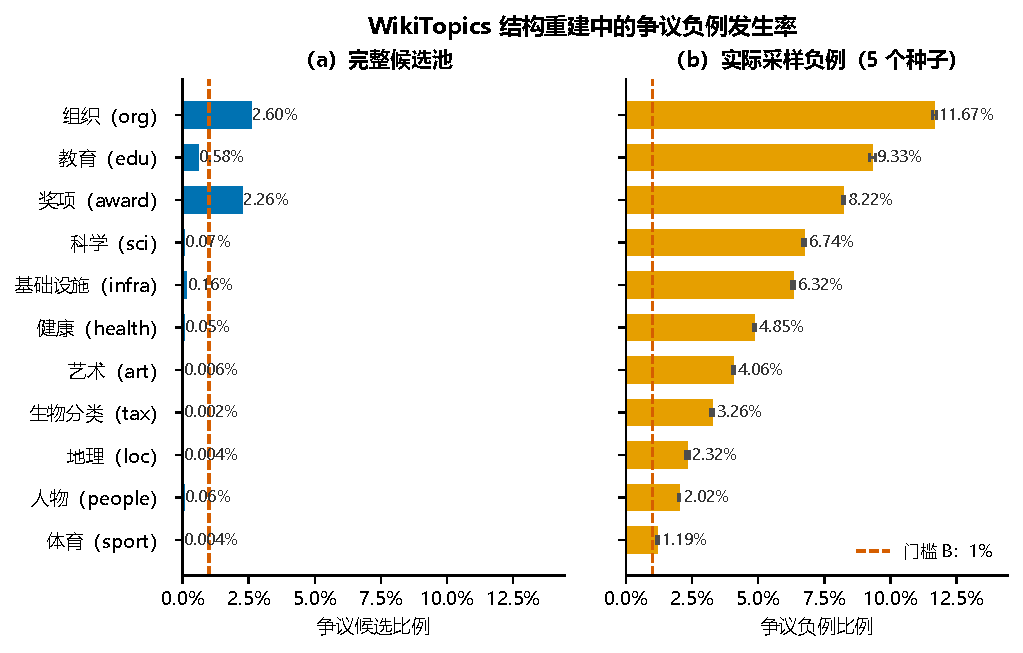
\includegraphics[width=0.92\linewidth]{../artifacts/figures/fig_prevalence.pdf}
\caption{候选池与实际采样负例中的争议比例。虚线为预先设定的 1\% 门槛。}
\label{fig:prevalence}
\end{figure}

门槛 B 的自动判定为“\GateBDecision”。该判定仅说明现象具有进入受控训练的规模，不表示策略2一定有效。

\subsection{四种监督处理的受控比较}

\begin{table}[H]
\centering
\small
\begin{tabular}{lccc}
\toprule
实验臂 & 答案可达率@10 & 全部最短路径召回率@10 & 选中路径曲线下面积\\
\midrule
\GateCMetricRows
\bottomrule
\end{tabular}
\caption{教育领域结构化代理实验的五种子均值 $\pm$ 标准差，表内均为百分数。}
\label{tab:gate-c}
\end{table}

\begin{figure}[H]
\centering
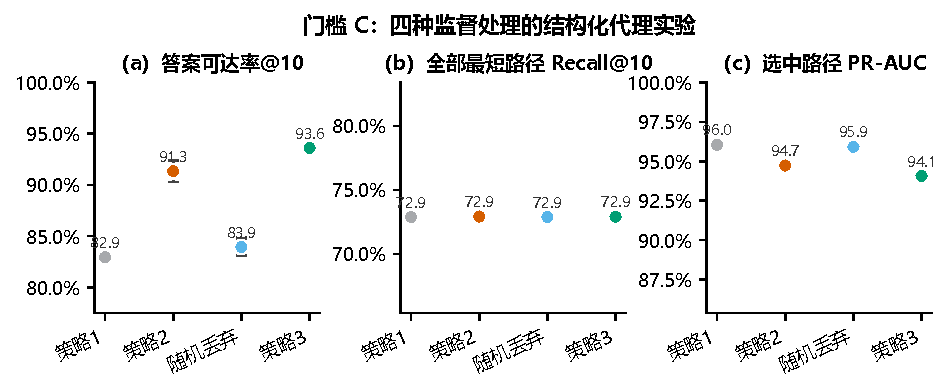
\includegraphics[width=\linewidth]{../artifacts/figures/fig_gate_c.pdf}
\caption{门槛 C 四个实验臂的主要结果。误差线表示五个随机种子的标准差。}
\label{fig:gate-c}
\end{figure}

策略2相对策略1的答案可达率@10配对差为 \VsStrategyOneDifference 个百分点，95\% 配对自助法区间为 [\VsStrategyOneCILow, \VsStrategyOneCIHigh]，共 \VsStrategyOnePairs 个“种子--问题”配对。相对随机丢弃的差为 \VsRandomDropDifference 个百分点，区间为 [\VsRandomDropCILow, \VsRandomDropCIHigh]，共 \VsRandomDropPairs 个配对。策略2相对策略1的选中路径曲线下面积差为 \StrategyTwoPrecisionDifference 个百分点。

\ifgatecpassed
三项预注册条件同时满足，门槛 C 判定为“\GateCDecision”。这意味着路径条件提供了超出样本数量变化的信号，但仍需门槛 D 的跨领域结果才能支持一般性结论。
\else
预注册条件没有同时满足，门槛 C 判定为“\GateCDecision”。因此，本研究按计划停止跨领域完整重训练。这个停止规则避免在观察教育领域结果后改变主要指标、筛选有利种子或扩大计算规模。
\fi

\section{讨论}

结构审计回答了“错误监督是否真实存在”，但它不能单独回答“删除这些监督是否改善模型”。门槛 C 进一步固定候选与特征，并加入随机丢弃对照，使策略2与单纯类别比例变化可区分。\ifgatecpassed 实验支持继续检验跨领域稳定性，但尚不证明原版端到端系统必然受益。\else 实验没有达到扩展标准；因此，不能仅凭争议负例比例较高就声称保守屏蔽优于公开基线。\fi

本文有三项边界。第一，门槛 C 是官方结构数据上的代理实验，不包含未发布的 GraphML、文本编码器和生成器，因而不能报告端到端答案精确匹配率。第二，路径一致是相对于观测图的结构性质；缺失边和伪边会分别拉长或缩短距离。第三，提案中的双人盲法语义标注需要独立人工标注者，本轮计算实验未获得该资源，因而没有把单个模型的判断伪装成人类一致性结果。本文对“语义有用证据占比”不作数值结论。

\section{结论}

本文把替代最短路径监督拆成发生率审计与受控因果比较。实现使用全局主题--答案成对距离，而不是较宽松的局部降距条件；策略1、策略2、策略3和随机丢弃共享候选、划分和特征。结果表明，争议候选会进入实际负采样，足以触发预设训练门槛。\ifgatecpassed 门槛 C 也满足扩展条件，但结论仍应等待跨领域门槛 D。\else 然而，策略2没有同时满足相对策略1、相对随机丢弃和精度保护三项条件，故当前证据不支持把它作为 HyperRAG 的有效改进。\fi

\section*{可复现性说明}

代码采用模块化目录，结构审计、数据准备、四臂训练、六卡调度、配对统计和绘图彼此分离。所有代码通过 GitHub 研究分支同步；服务器运行产物保留在独立实验目录。门槛 A 由 40 项单元测试覆盖，门槛 B 与门槛 C 的判定均由聚合脚本从原始运行结果自动生成，论文表格中的数字再由同一汇总文件生成，避免手工转录。

\bibliographystyle{plainnat}
\bibliography{../proposal/references}

\end{document}
